\chapter{Topology optimization in continua}
In the previous chapter, we learned how to transform a continuous elastic problem on a two-dimensional domain into a discrete problem using finite elements. 

\begin{objectives}{}{objectives_topology}
After studying this chapter and finishing the exercise, you should be able to 
\begin{itemize}[label=$\dots$]
    \item transfer solution methods from sizing problems to FEM-discretized problems
    \item solve for binary topologies using the SIMP approach
    \item discuss numerical problems in topology optimization
    \item apply filters to deal with numerical problems and manufacturing constraints
\end{itemize}
\end{objectives}

\section{Variable thickness sheet problem}
\label{sec:variable_thickness_sheet}
Let's consider a two-dimensional domain discretized with finite elements, in which we can adjust the thickness of each element. We may seek the best distribution of thicknesses $\mathbf{d}$ to minimize compliance $C$ with a constrained amount of material volume $V_0$. This problem can be formulated in analogy to the standard problem of sizing optimization stated in Equation \eqref{eq:size_optimization}: 

\begin{equation}
    \begin{aligned}
        \min_{\mathbf{d}} \quad & C(\mathbf{d}) = \mathbf{f} \cdot \mathbf{u}(\mathbf{d})\\
        \textrm{s.t.} \quad & \mathbf{d} \cdot \mathbf{A} - V_0 \le 0  \\
                            & \mathbf{d} \in \mathcal{D}\\
    \end{aligned}
    \label{eq:sheet_optimization}
\end{equation}

Mathematically, this problem is equivalent to the truss problem and can be solved in the same way: We formulate the Lagrangian
\begin{equation}
    \mathcal{L}(\mathbf{d}, \mu) = C(\mathbf{d}) + \mu \left( \mathbf{d} \cdot \mathbf{A} - V_0 \right) 
    \label{eq:lagrangian_sheet_optimization}
\end{equation}
and determine its derivative
\begin{equation}
    \frac{\partial \mathcal{L} (\mathbf{d}, \mu)}{\partial d_j} 
    = \frac{\partial C(\mathbf{d})}{\partial d_j} + \mu A_j 
\end{equation}
with 
\begin{equation}
    \frac{\partial C}{\partial d_j} = -2w_j(\mathbf{d}) = - \mathbf{u}_j(\mathbf{d})  \cdot \mathbf{k}^0_j \cdot \mathbf{u}_j(\mathbf{d}).
    \label{eq:sensitivity_sheet}
\end{equation}
In comparison to Equation \eqref{eq:compliance_sensitivity} for trusses with four degrees of freedom, the element displacement vector contains eight degrees of freedom for these 2D problems with linear quad elements ($\mathbf{u}_j \in \mathcal{R}^8, \mathbf{k}^0_j \in \mathcal{R}^{8\times 8}$). 

Just like the truss problem, the variable thickness sheet problem can be approximated using MMA with lower asymptotes only. Subsequently, it is solved with the dual method and a line search to find the Lagrange parameter $\mu$. The entire procedure is identical to Sections \ref{sec:sizing:mma} and \ref{sec:sizing:solution}, if we replace the truss cross sections $\mathbf{a}$ with element thicknesses $\mathbf{d}$ and the truss lengths $\mathbf{l}$ with element areas $\mathbf{A}$.

\begin{example}{Cantilever beam with MMA}{cantileveroptimizationexample}
    Consider a FEM cantilever beam from the previous example. Instead of just computing the displacements, we are now interested in finding the optimal thickness of each element given a volume constraint.

    We formulate the following algorithm to solve that problem: 
    \begin{enumerate}
        \item Define the cantilever FEM model with all nodes $\mathcal{N}$, elements $\mathcal{E}$, material property $E$, volume constraint $V_0$, design limits $\mathbf{d}^l, \mathbf{d}^u$ and the initial design choice $\mathbf{d}^0$.
        \item Compute the displacements $\mathbf{u}^k = \mathbf{u}(\mathbf{d}^k)$ by solving the FEM system for the current design $\mathbf{d}^k$.
        \item Compute the strain energies per area for all elements using the previously computed displacements   
        \begin{equation}
            w^k_j(\mathbf{d}^k) = \frac{1}{2}\mathbf{u}^k_j  \cdot \mathbf{k}^0_j \cdot \mathbf{u}^k_j
        \end{equation}
        \item Compute the lower asymptotes as $\mathbf{L}^k =\mathbf{d}^k - s (\mathbf{d}^u - \mathbf{d}^l)$ with $s \in (0,1)$ during the first two iterations and according to 
        \begin{equation}
            L^k_j = 
            \begin{cases}
                d^k_j - s  (d^{k-1}_j-L^{k-1}_j) & (d_j^k-d_j^{k-1})(d_j^{k-1}-d_j^{k-2}) < 0\\
                d^k_j - \frac{1}{\sqrt{s}}  (d^{k-1}_j-L^{k-1}_j) & \text{else}
            \end{cases}
        \end{equation}
        in the following iterations.
        \item Compute the lower move limit as 
        \begin{equation}
            \tilde{\mathbf{d}}^{l,k} = \max(\mathbf{d}_l,  0.9 \mathbf{L}^k + 0.1 \mathbf{d}^k)
        \end{equation}
        \item Evaluate the analytical solution
            \begin{align}
                \hat{d}_j(\mu) &= L_j^k + \sqrt{\frac{2 w_j (\mathbf{d}^k)
                (L^k_j-d^k_j)^2}{\mu A_j}} \\
                \mathbf{d}^* (\mu) &= \max\left(\tilde{\mathbf{d}}^{l,k}, \min \left(\hat{\mathbf{d}}(\mu), \mathbf{d}_u \right)\right)
            \end{align}
        \item Perform a line search to find the root $\mu^*>0$ in 
        \begin{equation}
            \frac{\partial \underline{\mathcal{L}}}{\partial \mu}(\mu) = \mathbf{A} \cdot \mathbf{d}^* (\mu) - V_0  = 0
        \end{equation}
        with Newton's method or bisection method. 
        \item Repeat with steps 2-7 until convergence or a maximum number of iterations is reached.
    \end{enumerate}

    The following image shows a result of the algorithm for the cantilever problem stated above. Black areas use the full maximum thickness $\mathbf{d}^u$ and white areas use the minimum thickness $\mathbf{d}^l$. The intermediate values are represented by different shades of gray.

    \begin{center}
        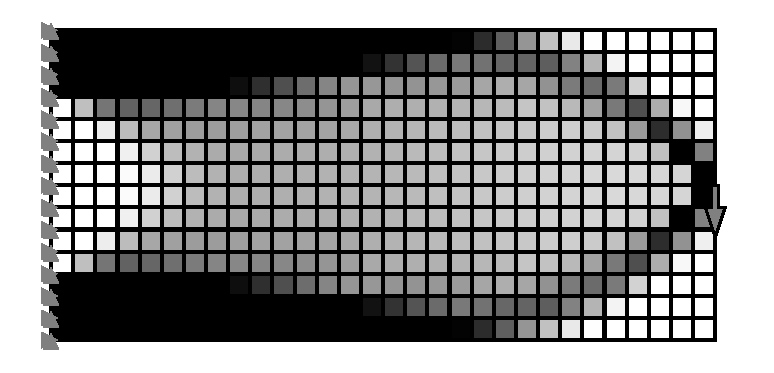
\includegraphics[width=\linewidth]{figures/cantilever_fem_optimized.pdf}
    \end{center}
    
\end{example}

\section{Solid isotropic material with penalization (SIMP)}
\label{sec:simp}
The problem stated in Equation \eqref{eq:sheet_optimization} is essentially a sizing optimization problem. In a topology optimization, we seek a material distribution, where each element is either completely filled or completely unfilled with material. We can formulate such a problem by reinterpreting the thickness variable as a normalized material density $\pmb{\rho}$, where $\rho_j=1$ indicates presence of material and $\rho_j=0$ indicates absence of material in element $j$. The stiffness of each element becomes a function of $\rho_j$, e.g. 
\begin{equation}
    \mathbb{C}(\rho_j)=
    \begin{cases}
        \mathbb{C} & \text{if} \quad \rho_j = 1 \\
        0          & \text{if} \quad \rho_j = 0
    \end{cases}
\end{equation}

Then, the problem statement reads
\begin{equation}
    \begin{aligned}
        \min_{\pmb{\rho}} \quad & C(\pmb{\rho}) = \mathbf{f} \cdot \mathbf{u}(\pmb{\rho})\\
        \textrm{s.t.} \quad & \pmb{\rho} \cdot \mathbf{V} - V_0 \le 0  \\
                            & \rho_j \in \{0, 1\}\\
    \end{aligned}
    \label{eq:topology_optimization}
\end{equation}

where the only change compared to Equation \eqref{eq:sheet_optimization} is the discrete nature of the design variables $\pmb{\rho}$ and the name of the design variables. Hence, we formulate the Lagrangian analogously to Equation \eqref{eq:lagrangian_sheet_optimization} as 
\begin{equation}
    \mathcal{L}(\pmb{\rho}, \mu) = C(\pmb{\rho}) + \mu \left( \pmb{\rho} \cdot \mathbf{A} - V_0 \right).
    \label{eq:lagrangian_topology_optimization}
\end{equation}

Unfortunately, the binary problem is notoriously hard to solve, because we cannot compute gradients on the solution and testing all solutions is computationally inaccessible. Hence we try to formulate a continuous relation between stiffness and normalized density that still results in a binary result. One such formulation is called \emph{Solid Isotropic Material with Penalization} (SIMP) and denoted as 
\begin{equation}
    \mathbb{C}(\rho_j)= \rho_j^p \mathbb{C}
\end{equation}
with a penalization parameter $p \ge 1$. 
The effect of penalization is shown in Figure \ref{fig:simp} for typical values of $p$. We may observe for $p>1$ that the stiffness per invested material is unattractive for intermediate density values. For example, choosing $\rho_j=0.5$ adds half an element volume to the total volume, but contributes only a quarter of the stiffness compared to a fully filled element. An optimization that tries to minimize compliance for a given volume will therefore rather favor elements that provide the full stiffness benefit ($\rho=1$) or do not count towards the constraint ($\rho=\rho^l$). 

\begin{figure}[!htpb]
    \centering
    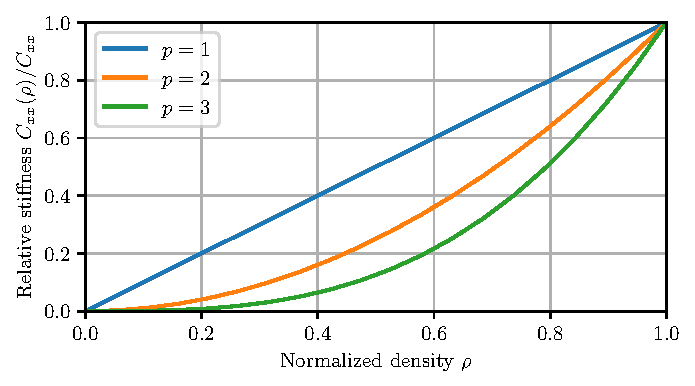
\includegraphics[width=0.9\textwidth]{figures/simp.pdf}
    \caption{Penalization factors in SIMP.}
    \label{fig:simp}
\end{figure}

Incorporating the SIMP method to the optimization is straight-forward. We just need to adjust the sensitivity (see Equation \ref{eq:sensitivity_sheet}) slightly to
\begin{equation}
    \frac{\partial C}{\partial \rho_j} = -2 p \rho_j^{p-1} w_j(\pmb{\rho}^k) = - p \rho_j^{p-1} \mathbf{u}_j(\pmb{\rho})  \cdot \mathbf{k}^0_j \cdot \mathbf{u}_j(\pmb{\rho}).
    \label{eq:sensitivity_topology}
\end{equation}

\begin{example}{Cantilever beam with MMA and SIMP}{cantileversimpoptimizationexample}
    Consider a FEM cantilever beam from the previous example. We only adjust the solution in Step 6 towards 
    \begin{equation}
        \hat{\rho}_j(\mu) = L_j^k + \sqrt{\frac{-2p \rho_j^{p-1} w_j(\pmb{\rho}^k)
        (L^k_j-d^k_j)^2}{\mu A_j}}
    \end{equation}
    and we end up with the following solution:
    \begin{center}
        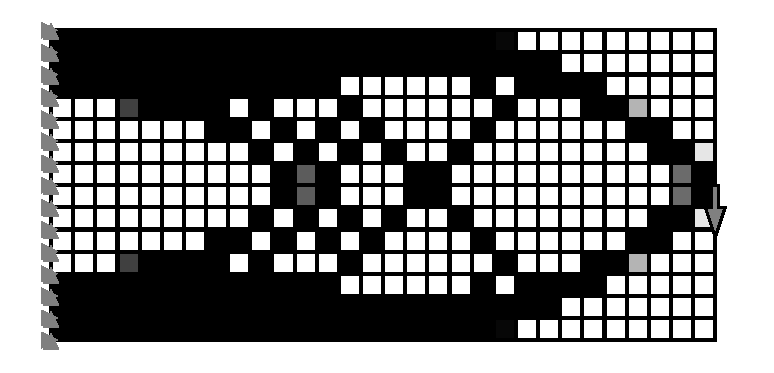
\includegraphics[width=\linewidth]{figures/cantilever_fem_optimized_binary.pdf}
    \end{center}
\end{example}

\section{Filters}
Obviously, the SIMP approach helps us to find a binary solution of the discretized problem stated in Equation \eqref{eq:topology_optimization}. However, we may ask ourselves if there is a unique solution to this problem independent of discretization. And it turns out, the answer is no: You can improve any given design by replacing it with finer structures in a process that goes on indefinitely \cite{Christensen2008}. 
In addition to the theoretical non-existence of a solution, this also means that our solution is \emph{mesh-dependent}: If we want to refine the solution, we may end up with a totally different solution. 

\begin{example}{Cantilever beam mesh dependency}{cantileverdiscoptimizationexample}
    We can increase the resolution of the previous examples to achieve better compliance results. However, this demonstrates the mesh-dependence of the solution and we observe structures which might be difficult to manufacture.
    
    Finer resolution:
    \begin{center}
        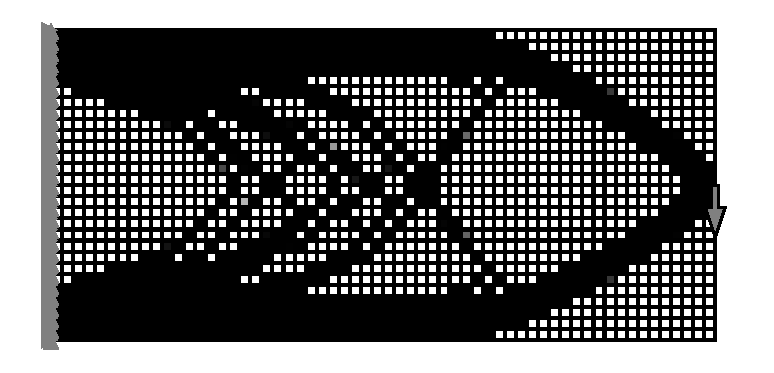
\includegraphics[width=\linewidth]{figures/cantilever_fem_optimized_binary_fine.pdf}
    \end{center}
    
    Even finer resolution:
    \begin{center}
        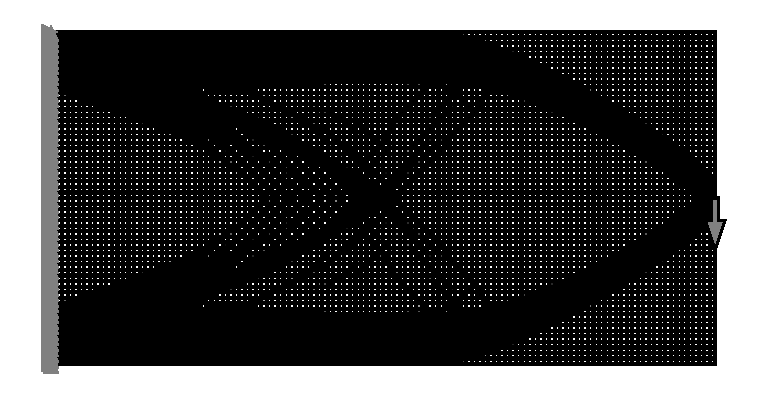
\includegraphics[width=\linewidth]{figures/cantilever_fem_optimized_binary_extra_fine.pdf}
    \end{center}
\end{example}

Even if we were to accept mesh dependence and the theoretical problems, we are still left with challenges in the resulting designs. First of all, fine structures may be hard to manufacture. Even additive manufacturing methods are limited to some minimal structure size. Secondly, we may observe checkerboard-like patterns on the structure. These are numerical artifacts from the fact that we use linear shape functions which lead to an overestimation of the stiffness for that configuration.

We can address all these problems with the introduction of filters as a regularization \cite{Harzheim2014, Lazarov2011}. There are two traditional approaches for mesh-independent filtering: \emph{density filtering} and \emph{sensitivity filtering}. In density filtering, we replace the density $\pmb{\rho}$ with a weighted sum of neighboring densities, and use this filtered density $\tilde{\pmb{\rho}}$ in the stiffness evaluation
\begin{equation}
    \mathbb{C}(\rho_j)= \tilde{\rho}_j^p(\pmb{\rho}) \mathbb{C}.
\end{equation}
The filtered density is computed according to 
\begin{equation}
    \tilde{\rho}_j (\pmb{\rho}) = \frac{\sum_i H_{ji} A_i \rho_i}{\sum_i H_{ji} A_i}
\end{equation}
with a distance weighting matrix
\begin{equation}
    H_{ji} = 
    \begin{cases}
        R-\lVert \mathbf{x}_i - \mathbf{x}_j\rVert & \text{if} \quad \lVert \mathbf{x}_i - \mathbf{x}_j\rVert \le R \\
        0 & \text{else},
    \end{cases}
\end{equation}
where $R$ describes the filter radius. This filter results in a structural weakening of structures finer than $R$, as they get smeared with neighboring empty elements. Hence, the filter solves the mesh-dependency problem, prevents structures that cannot be manufactured and prevents checkerboard patterns. However, we need to account for the filter during sensitivity computation by 
\begin{equation}
    \frac{\partial C}{\partial \rho_j} 
    = \frac{\partial C}{\partial \tilde{\rho}_m} \frac{\partial \tilde{\rho}_m}{\partial \rho_j}
    = \frac{\partial C}{\partial \tilde{\rho}_m}  \frac{H_{jm} A_m }{\sum_i H_{ji} A_i}
\end{equation}
and in the volume constraint.

An alternative to filtering densities is filtering of sensitivities. We may compute the filtered sensitivity as
\begin{equation}
    \widetilde{\frac{\partial C}{\partial \rho_j}} = \frac{1}{\rho_j} \frac{\sum_i H_{ji} A_i \rho_i \frac{\partial C}{\partial \rho_i} }{\sum_i H_{ji} A_i}
\end{equation}
which is a purely heuristic concept, i.e. there is no mathematical proof for this filter to work \cite{Sigmund1998}. However, we can implement this formulation simply by replacing the sensitivities in \eqref{eq:sensitivity_topology} with filtered sensitivities. This is very efficient, simple to implement and experience shows that this filter works quite well.

\begin{example}{Cantilever beam  with sensitivity filtering}{cantileverfilterexample}
    The following images show the optimized cantilever beams from previous examples with enabled sensitivity filtering. Filtering prevents small structures and regularizes the problem such that we achieve similar optimal designs for different mesh sizes.

    Previous example:
    \begin{center}
        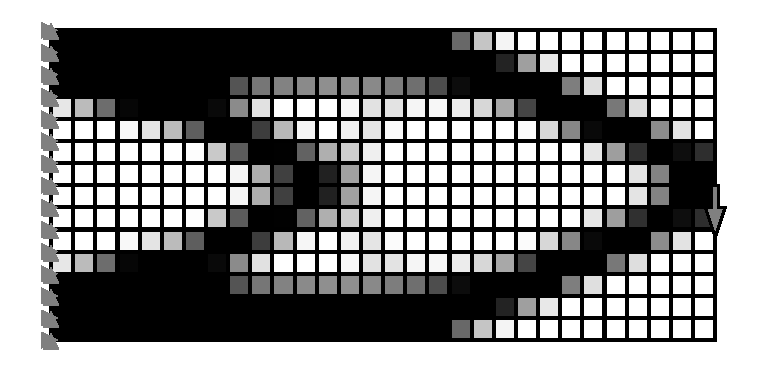
\includegraphics[width=\linewidth]{figures/cantilever_fem_optimized_binary_filtered.pdf}
    \end{center}
    
    Finer resolution:
    \begin{center}
        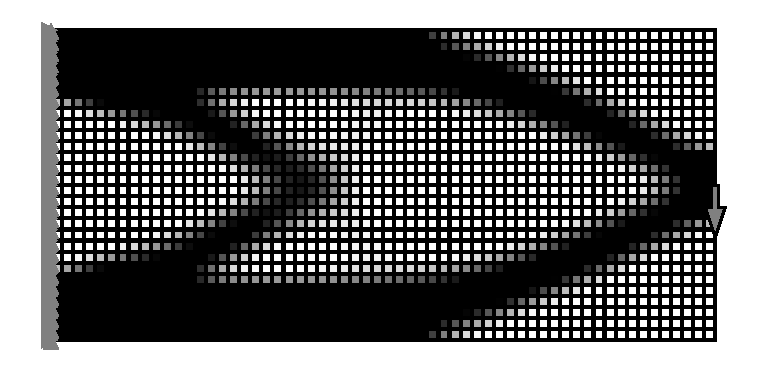
\includegraphics[width=\linewidth]{figures/cantilever_fem_optimized_binary_fine_filtered.pdf}
    \end{center}
    
    Even finer resolution:
    \begin{center}
        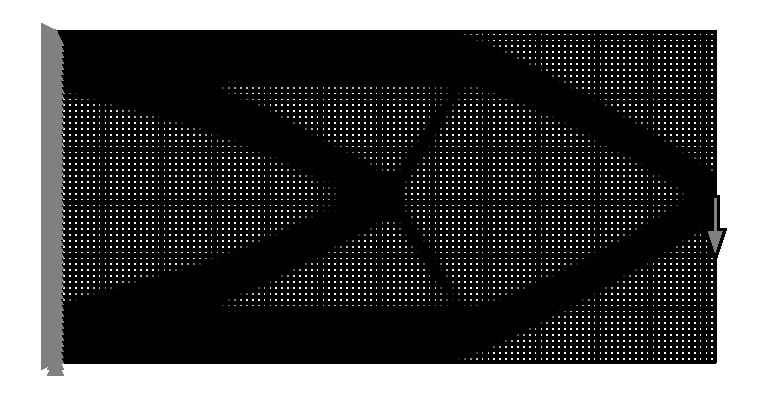
\includegraphics[width=\linewidth]{figures/cantilever_fem_optimized_binary_extra_fine_filtered.pdf}
    \end{center}
\end{example}

There is one more challenge in the SIMP formulation of the standard topology optimization problem: For $p>1$, the problem is not convex anymore and different starting points may result in different local minima \cite{Christensen2008}. A strategy to cure termination at non-global minima is a gradual increase of $p$ starting from $p=1$ and using multiple starting points $\pmb{\rho}^0$.

\section{Optimality criteria}
The solution via MMA is in line with the previous chapters of this manuscript and is able to solve arbitrary problems beyond the compliance minimization stated in problem \eqref{eq:topology_optimization}. Historically, this specific problem was first solved with the \emph{optimality criteria method} instead of convex approximations. The idea here is that we can use the gradient of the Lagrangian given in Equation \eqref{eq:lagrangian_topology_optimization}
\begin{equation}
    \frac{\partial \mathcal{L} (\pmb{\rho}, \mu)}{\partial\rho_j} 
    = \frac{\partial C(\pmb{\rho})}{\partial \rho_j} + \mu A_j = 0
\end{equation}
to formulate an optimality condition
\begin{equation}
    G_j = \frac{-\frac{\partial C(\pmb{\rho})}{\partial \rho_j}}{\mu A_j} = \frac{p \rho_j^{p-1} \mathbf{u}_j(\pmb{\rho})  \cdot \mathbf{k}^0_j \cdot \mathbf{u}_j(\pmb{\rho})}{\mu A_j} = 1
\end{equation}
that must be fulfilled at the optimum whenever a variable does not reach its bounds.
A heuristic algorithm can now compute $G_j$ and adjust $\rho_j$ such that $G_j$ approaches 1. We may realize that increasing $\rho_j^k$ increases the stiffness and hence decreases the displacement for a given load. Consequently, increasing $\rho_j$ decreases $G_j$ and vice versa. Hence, an update rule 
\begin{equation}
    \hat{\rho}_j^{k+1} = \left(G_j^k\right)^\xi \rho_j^k 
\end{equation}
drives the solution towards the optimal point $\rho_j^*$, where $G^*_j=1$. The exponent $\xi \in (0,1]$ stabilizes the algorithm with typical values being $\xi=0.5$ \cite{Harzheim2014}. 

In addition, we employ move limits 
\begin{align}
    \rho_j^{l,k} &= \max \left(\rho_j^l, (1-m)\rho_j^k \right) \\
    \rho_j^{u,k} &= \min \left(\rho_j^u, (1+m)\rho_j^k \right)
\end{align}
to compute the next value as 
\begin{equation}
    \rho_j^{k+1} = \max \left( \min \left(\hat{\rho}_j^{k+1}, \rho_j^{u,k} \right), \rho_j^{l,k} \right).
\end{equation}
The move limits reduce the maximum step width and account for bounds on the design variables. 

To compute $G_j$, we need to determine the value of the Lagrange multiplier $\mu$. For the compliance problem, we can intuitively assume that the stiffest structure will use all material and consequently, that the volume constraint will be active. the Lagrange multiplier may be found with the bisection method on the feasibility condition
\begin{equation}
    \frac{\partial \mathcal{L}}{\partial \mu} = \pmb{\rho}(\mu) \cdot \mathbf{A} - V_0 = 0.
\end{equation}

\begin{example}{Algorithm with optimality criteria and SIMP}{ocexample}
    Consider a FEM cantilever beam from the previous example. 

    We formulate the following algorithm to solve that problem: 
    \begin{enumerate}
        \item Define the cantilever FEM model with all nodes $\mathcal{N}$, elements $\mathcal{E}$, material property $E$, volume constraint $V_0$, design limits $\mathbf{d}^l, \mathbf{d}^u$ and the initial design choice $\mathbf{d}^0$.
        \item Compute the displacements $\mathbf{u}^k = \mathbf{u}(\mathbf{d}^k)$ by solving the FEM system for the current design $\mathbf{d}^k$.
        \item Apply the bisection method to find the root of 
            \begin{equation}
                g(\mu) = \pmb{\rho}^{k+1}(\mu) \cdot \mathbf{A} - V_0
            \end{equation}
        with 
        \begin{equation}
            \pmb{\rho}^{k+1}(\mu) = \max \left( \min \left(\left(G_j^k(\mu)\right)^\xi \rho_j^k , \rho_j^{u,k} \right), \rho_j^{l,k} \right).
        \end{equation}
        \item Repeat with steps 2-3 until convergence or a maximum number of iterations is reached.
    \end{enumerate}
\end{example}

In addition to the density-based method shown so far, topology optimization may also be performed with \emph{Level-Set methods} and empirical growth rules like \emph{Soft Kill Option}. These methods are not addressed in this lecture.

\section{Interpretation}
Finally, it is important to note that topology optimizations provide only design suggestions and not a design than can be readily manufactured. With the current state of research, we always need to interpret the result in the context of a manufacturing method.

\begin{example}{Cantilever beam  interpretation}{cantileverinterpretationexample}
    We may project the solution of a topology optimization problem to a canvas in a CAD software and use it as a guide to sketch an actual component:
    \begin{center}
        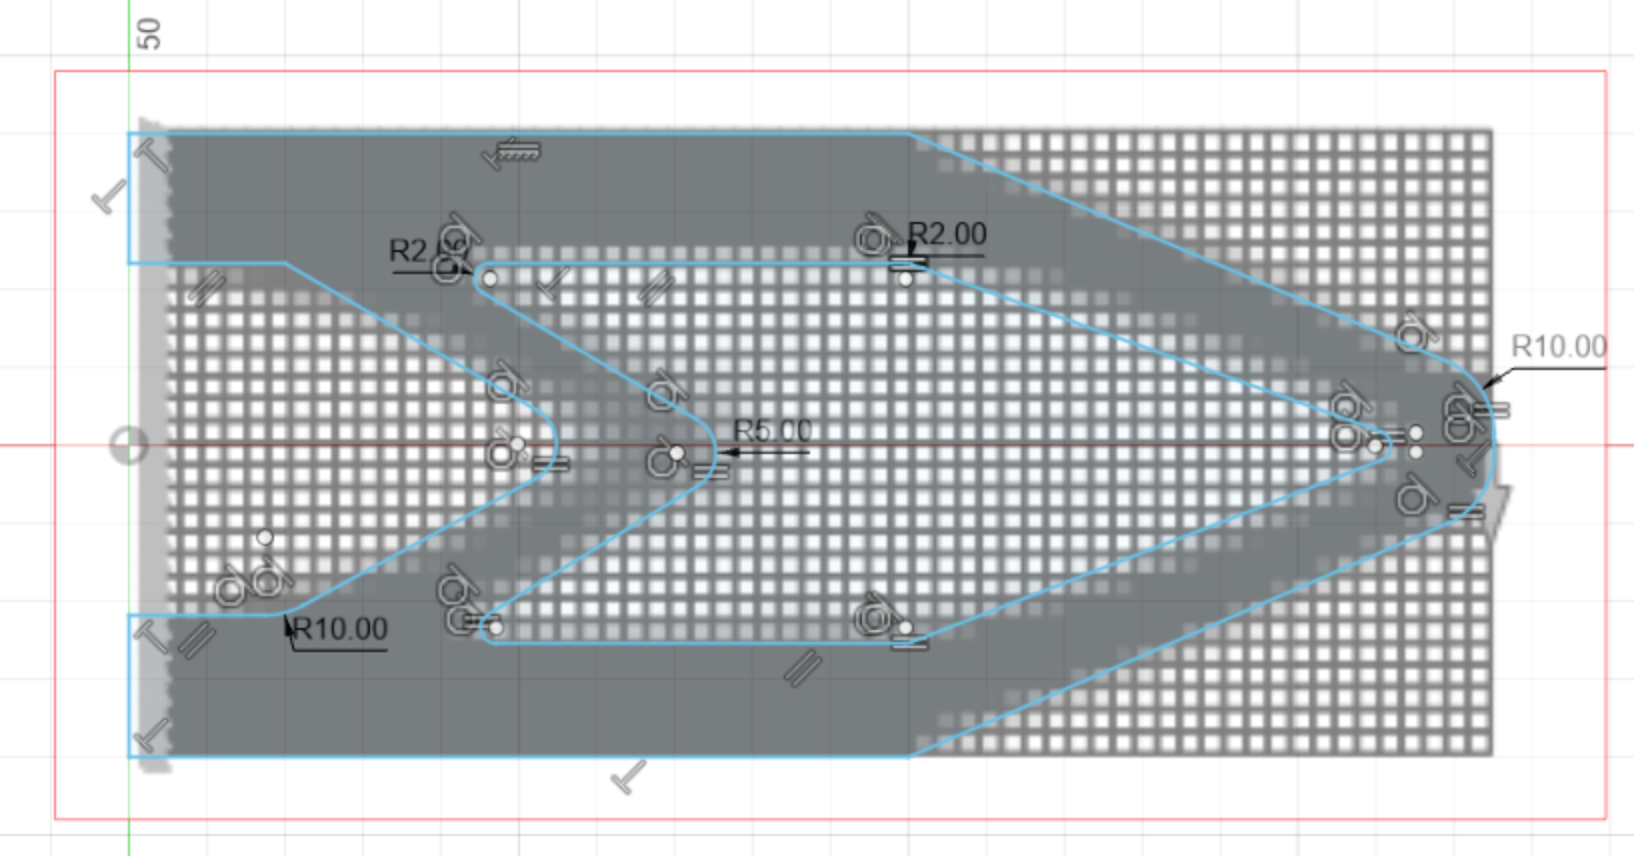
\includegraphics[width=\linewidth]{figures/cantilever_template.png}
    \end{center}
    
    This is an interpretation of the cantilever beam as a sheet metal design:
    \begin{center}
        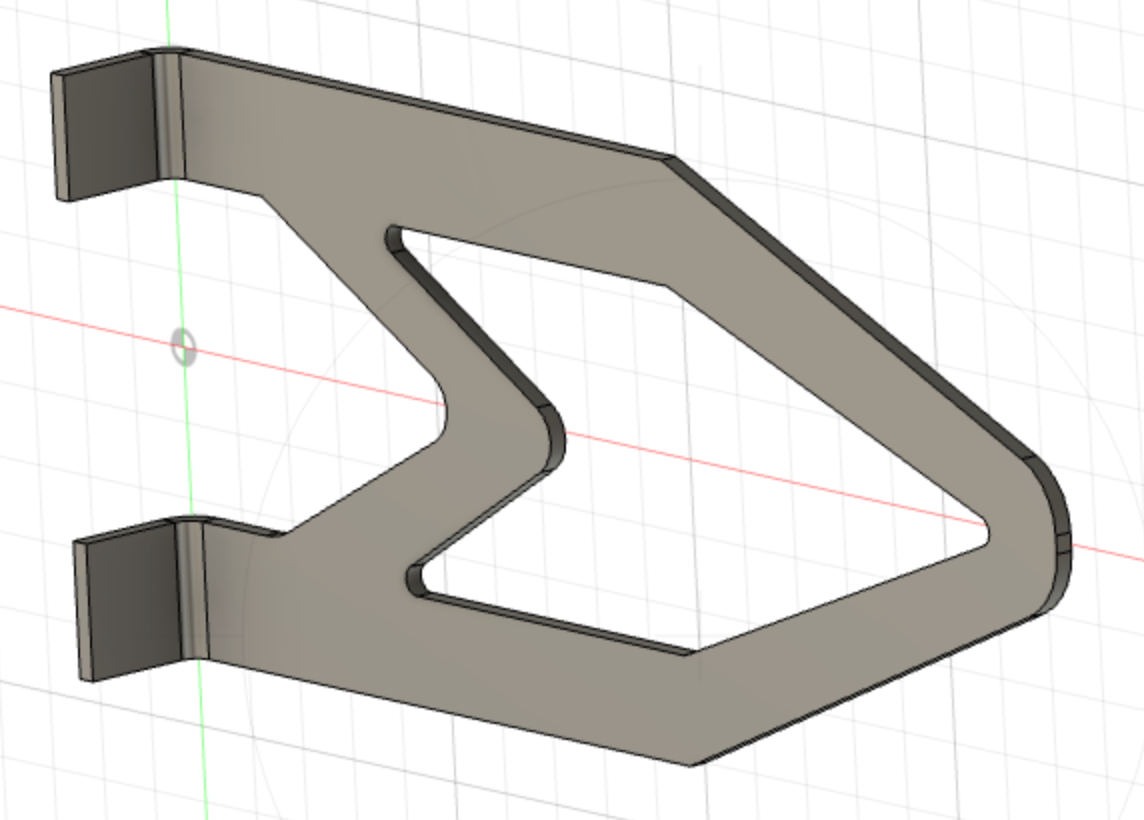
\includegraphics[width=\linewidth]{figures/cantilever_design.png}
    \end{center}
\end{example}


\bibliographystyle{unsrtnat}
\bibliography{literature} 